\documentclass[a4paper, 12pt]{article}
\usepackage[a4paper,top=1.5cm, bottom=1.5cm, left=1cm, right=1cm]{geometry}
\usepackage{cmap}					
\usepackage{mathtext} 				
\usepackage[T2A]{fontenc}			
\usepackage[utf8]{inputenc}			
\usepackage[english,russian]{babel}
\usepackage{multirow}
\usepackage{graphicx}
\usepackage{wrapfig}
\usepackage{tabularx}
\usepackage{float}
\usepackage{longtable}
\usepackage{hyperref}
\hypersetup{colorlinks=true,urlcolor=blue}
\usepackage[rgb]{xcolor}
\usepackage{amsmath,amsfonts,amssymb,amsthm,mathtools} 
\usepackage{icomma} 
\usepackage{euscript}
\usepackage{mathrsfs}
\usepackage{enumerate}
\usepackage{caption}
\usepackage{enumerate}
\mathtoolsset{showonlyrefs=true}
\usepackage{graphicx}
\usepackage{caption}
\usepackage{subcaption}
\usepackage[europeanresistors, americaninductors]{circuitikz}
\DeclareMathOperator{\sgn}{\mathop{sgn}}

\newcommand*{\hm}[1]{#1\nobreak\discretionary{}
	{\hbox{$\mathsurround=0pt #1$}}{}}

\newcommand{\RomanNumeralCaps}[1]
    {\MakeUppercase{\romannumeral #1}}

\title{\textbf{Определение модуля кручения (1.3.2)}}
\author{Манро Эйден}
\date{}

\begin{document}

\maketitle
	      	
    \begin{center}
    \section*{Введение}    
    \end{center}


    \noindent \textbf{Цель работы:} измерение углов закручивания в зависимости от приложенного момента сил, расчёт модулей кручения и сдвига при статическом закручивании стержня, определение тех же модулей для проволоки по измерениям периодов крутильных колебаний подвешенного на ней маятника (динамическим методом).

    \bigskip

    \noindent \textbf{Оборудование:} в первой части: исследуемый стержень, отсчётная туба со шкалой, рулетка, штангенциркуль, набор грузов; во второй части: проволока из исследуемого материала, грузы, секундомер, штангенциркуль, линейка, рулетка.
    
    \bigskip

    \begin{center}    
    \subsection*{Теоретические сведения}
    \end{center}
    
    При закручивании цилиндрических стержней круглого сечения распределение деформаций
    и напряжений одинаково по длине стержня только вдали от мест, где прикладываются закручивающие моменты.
    Для этих областей можно считать, что каждое поперечное сечение поворачивается поворачивается как жесткое,
    то есть частички материала не сходят с радиальных линий, на которых они были в начале, и все
    эти линии поворачиваются на один и тот же угол. Такое напряженное состояние назвается чистым кручением.\\

    При такой деформации любая прямая линия, проведенная до закручивания цилиндра по частицам материала и параллельная оси симметрии,
    при закручивании превращается в спираль (винтовую линию). \\

    Покажем, что касательное напряжение напряжение в поперечном сечении увеличивается пропорцианально расстоянию до оси вращения.
    Рассмотрим в цилиндре колечко бесконечно малой толщиной $dr$ и высоты $dl$. При закручивании верхнее колечко поворачивается относительно 
    нижнего на угол $d\varphi$, а образующая наклоняется на угол $\alpha$. Тогда при малых углах справедливо соотношение:

    \bigskip
    
    \begin{equation}
        \alpha dl= r d\varphi 
    \end{equation}

    \bigskip

    Касательное наряжение $\tau $ связано с углом $\alpha$ линейной зависимостью через модуль сдвига $G$, и следовательно растет с увеличением расстоянием от оси:

    \bigskip
    
    \begin{equation}
        \tau = G\cdot \alpha =Gr\frac{d\varphi}{dl} 
    \end{equation}

    \bigskip

    Эти касательные напряжения создают момент сил относительно оси цилиндра:


    \bigskip

    \begin{equation}
        dM=2\pi r dr \cdot r\cdot \tau  
    \end{equation}

    \bigskip
    
    Интегрируя это выражение по всем колечкам от оси цилиндра до его радиуса R находим суммарный
    момент сил:

    \bigskip

    \begin{equation}
        M = \frac{\pi G R^{4}}{2} \frac{d \varphi }{d l} 
    \end{equation}

    \bigskip

    Так как момент сил не меняется по длине цилиндра. Тогда для связи приложенного
    момента сил $M$ и угла поворота $\varphi$ поперечных сечений цилиндра имеем:

    \bigskip

    \begin{equation}
        M=\frac{\pi R^{4}G}{2l}\varphi=f \varphi
    \end{equation}

    \bigskip

    Где $f$ - модуль кручения связанный с модулем сдвига $G$ соотношением:

    \bigskip
    
    \begin{equation}
        G=\frac{2l}{\pi R^{4}}f
    \end{equation}

    \bigskip

    \begin{center}
        \subsection*{Погрешности}
    \end{center}

    \begin{center}
        Случайая погрешность измерений:

    \bigskip
    
    \begin{equation}
        \sigma_\text{сл}=\sqrt{\frac{1}{N\left( N - 1 \right)}\sum_{i=1}^{N}\left( x_\text{ср} - x_i \right)^2 }
    \end{equation}
    
    \bigskip
    
    
    \begin{itemize}
        
        \item Весы: $\Delta_{\text{в}} = 0,01 \text{ г}$
        \item Линейка: $\Delta_{\text{л}} = 0,05 \text{ см}$
        \item Штангенциркуль: $\Delta_{\text{шт}} = 0,1 \text{ мм}$
    
    \end{itemize}
    
    \end{center}
    
    \begin{center}
        \section*{\RomanNumeralCaps{1}. Определение модуля кручения стержня статическим методом}     
    \end{center}

    \bigskip

    \begin{center}
        \subsection*{Экспериментальная установка}
    \end{center}

    Эту часть работы будем проводить на установке, схематично изображённой ниже. Она состоит из вертикально расположенного стержня С, верхний конец которого прочно закреплён на стойке, а нижний соединён с диском Д. Момент $M$, закручивающий стержень создают две навитые на диск и перекинутые через блоки Б нити, к концам которых подвешиваются одинаковые грузы Г. Диск снабжён зеркальцем З. Для того, чтобы узнать угол поворота диска, нужно направить зрительную трубу на зеркальце и сделать так, чтобы в неё была чётко видна шкала, укреплённая на том же штативе, что и трубка. По изменению положения шкалы можно определить угол закручивания $\varphi$.

    \begin{figure}[H]
        \begin{center}
            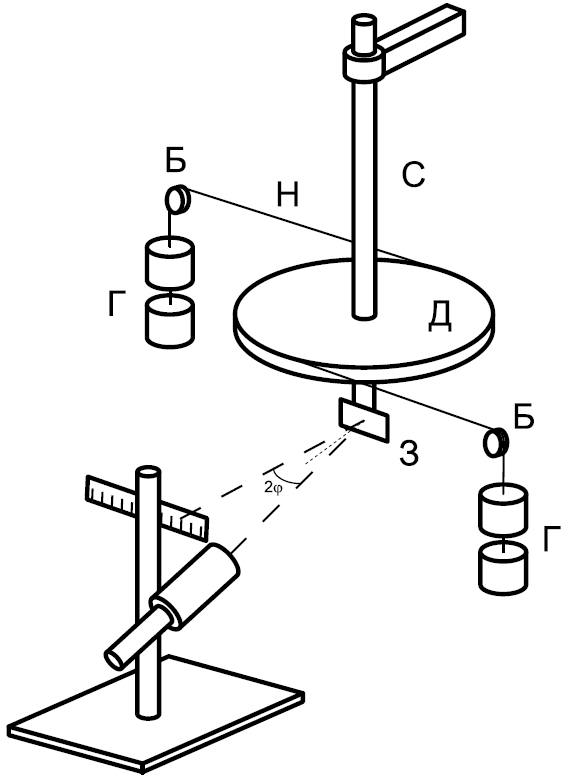
\includegraphics[scale=0.40]{ust1.png}
            \begin{center}
                \caption{Схема установки \RomanNumeralCaps{1}}
            \end{center}
            \label{graphic1b}
        \end{center}
    \end{figure}

    \begin{center}
        \subsection*{Ход работы}
    \end{center}

    \begin{center}
    
    \begin{table}[h!]
        \begin{center}
        \begin{tabular}{|c|c|}
        \hline \hline
        $d_{\text{ст}}$, мм & 6,00 $\pm$ 0,01  \\ \hline
        $d_{\text{д}}$, мм  & 107,2 $\pm$ 0,01    \\ \hline
        $L$, см             & 157,0 $\pm$ 0,5     \\ \hline
        $l$, см             & 137,0 $\pm$ 0,1 \\ \hline
        $m_{0}$, г         & 50,0 $\pm$ 0,1   \\ \hline \hline
        \end{tabular}
        \caption{Размеры установки}
        \end{center}
    \end{table}


    \begin{table}[h!]
        \begin{center}
        \begin{tabular}{|c|c|c|c|c|c|c|c|c|}
        \hline \hline
        $m, \text{ гр}$ &  $ \Delta l_1 \uparrow, \text{ см}$ & $ \Delta l_1 \downarrow, \text{ см}$ & $ \Delta l_2 \uparrow, \text{ см}$ & $ \Delta l_2 \downarrow, \text{ см}$ &  $ \Delta l_3 \uparrow, \text{ см}$ & $ \Delta l_3 \downarrow, \text{ см}$ & $\Delta l_{\text{ср}}, \text{ см}$ & $\sigma_{\Delta l}, \text{ см} $ \\ \hline \hline
          50  & 3,0  & 2,7  & 3,0  & 2,6  & 2,8  & 2,9  & 2,833  & 0,067 \\ \hline
          100 & 5,3  & 5,1  & 5,4  & 5,3  & 5,2  & 5,5  & 5,300  & 0,057 \\ \hline
          150 & 8,3  & 8,1  & 8,4  & 7,8  & 8,0  & 8,0  & 8,100  & 0,089 \\ \hline
          200 & 10,5 & 10,2 & 10,5 & 10,2 & 10,1 & 10,5 & 10,333 & 0,076 \\ \hline
          300 & 15,8 & 16,2 & 16,0 & 16,5 & 16,2 & 16,1 & 16,133 & 0,095 \\ \hline
          400 & 20,5 & 20,5 & 20,3 & 20,3 & 20,3 & 20,3 & 20,366 & 0,042 \\ \hline  
        \hline 
        \end{tabular}
    \caption{Экспериментальные данные}
    \end{center}
    \end{table}

    \bigskip

    Момент силы грузов будет равен:
    \begin{equation}
        M = (m_{1}+m_{0})gR_{\text{диск}} + (m_{2}+m_{0})gR_{\text{диск}} \approx 2(m+m_{0})gR_{\text{диск}} = (m+m_{0})gd_{\text{диск}}
    \end{equation}

    Угол поворота будет равен:
    \begin{equation}
        \varphi = arctg(\frac{\Delta l}{L}) \approx \frac{\Delta l}{L} (\Delta l \ll L).
    \end{equation}
    
    \end{center}

    \newpage

    \begin{table}[h!]
    \begin{center}
        \begin{tabular}{|c|c|c|c|}
        \hline \hline
        $ M, \text{ кг}\frac{\text{м}^2}{\text{с}^2}$ & $ \varphi $ & $\sigma_{M}$ & $\sigma_{\varphi}$ \\ \hline \hline
        0,105 & 0,01804 & 0,001 & 0,00043 \\ \hline
        0,157 & 0,03375 & 0,001 & 0,00036 \\ \hline
        0,210 & 0,05159 & 0,001 & 0,00056 \\ \hline
        0,262 & 0,06581 & 0,001 & 0,00048 \\ \hline
        0,368 & 0,10275 & 0,001 & 0,00060 \\ \hline
        0,473 & 0,12972 & 0,001 & 0,00026 \\ \hline \hline
        \end{tabular}
    \caption{Данные для графика}
    \end{center}
    \end{table}

    \begin{figure}[H]
        \centering
        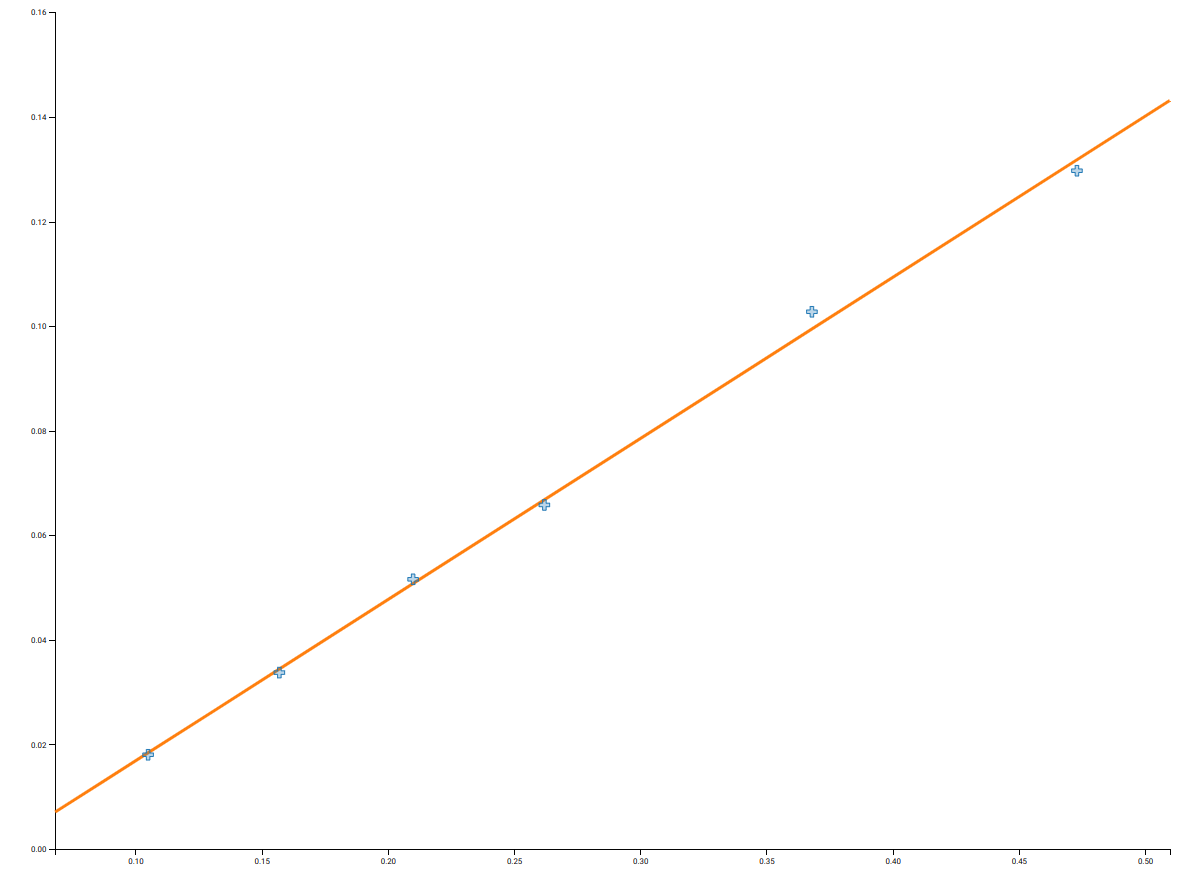
\includegraphics[scale = 0.4, angle=90]{graph1.png}
        \caption{Зависимость $\varphi = k \cdot M$}
    \end{figure}

    \newpage

    \begin{center}
        
    Получаем, что:

    \bigskip
    
    \begin{equation}
        k = (0,239 \pm 0,016) \frac{\text{рад}}{\text{Н} \cdot \text{м}}, \;
        \varepsilon_{k} = 6,6 \%
    \end{equation}

    \bigskip

    $f = \frac{1}{k} = (4,184 \pm 0,276) \frac{\text{Н} \cdot \text{м}}{\text{рад}}, \; \varepsilon_{f} \approx 6,6\%$.
    \begin{equation}
        G=\frac{2l}{\pi R^{4}}f
    \end{equation}

    \bigskip
    
    Погрешность:

    \bigskip
    
    \begin{equation}    
    \varepsilon_{G} = \sqrt{(\varepsilon_{f})^2 + (\varepsilon_{l})^2 + (4\varepsilon_{R})^2}
    \end{equation}

    \bigskip
    
Итого: \underline{$\varepsilon_{G} = 6,62\%$, $G = 0,442$ ГПа}

\end{center}

\newpage

\section*{\RomanNumeralCaps{2}. Определение модуля сдвига при помощи крутильных колебаний}
    
\begin{center}
\subsection*{Теоретические сведения}
\end{center}

В системе можно возбудить крутильные колебания. Вращение стержня с закрепленными
на нем грузиками вокрунг вертикальной оси проиходит под действием упругого момента $M$.
С учетом выражения для момента $M$ получим, что это вращение описывается уравнением колебаний:
\begin{equation}
    I\frac{d^2 \varphi }{d t^2} + f \varphi =0
\end{equation}
Следовательно период кoлебаний системы связан с расстоянием $r$ от оси вращения до грузов и
моментом инерции стержня $I_0$ следующим образом:
\begin{equation}
    \omega^2 = \frac{f}{I}
\end{equation}

\begin{equation}
    T = 2\pi\sqrt{\frac{I}{f}}
\end{equation}

\bigskip

Эти зависимости были получены для незатухающих колебаний. Поэтому для их применения необходимо убедиться, что в рассматриваемой системе диссипативными силами можно пренебречь. Для этого стоит убедиться, что период колебаний не зависит от начальной амплитуды и что амплитуда уменшьется не более чем в 2 раза после около 10 колебаний.\\
Применяя Теорему Гюйгенса-Штейнера:

\bigskip

\begin{equation}
    T^2 = (2\pi)^2\frac{I}{f} = (2\pi)^2\frac{I_{0}}{f} + (2\pi)^2\frac{(m_{1}+m_{2})r^2}{f},
\end{equation}

\bigskip

\begin{center}
где $I_{0} = \frac{1}{4}mr^2 + \frac{1}{12}ml^2 + \frac{1}{4}ml^2 = \frac{1}{4}mr^2 + \frac{1}{3}ml^2$
\end{center}

\bigskip

\begin{center}
\subsection*{Экспериментальная установка}
\end{center}

Экспериментальная установка, используемая в этой части работы,
изображена на рис. 1 и состоит из длинной вертикально висящей право-
локи П, к нижнему концу которой прикреплен горизонтальный метал-
лический стержень С с двумя симметрично расположенными грузами
Г. Их положение на стержне можно фиксировать. Верхний конец право-
локи зажать в цангу и при помощи специального приспособления может
вместе с цангой поворачиваться вокруг вертикальной оси. Таким спо-
собом в системе можно возбуждать крутильные колебания. Вращение
стержня С с закрепленными на нем грузами Г вокруг вертикальной
оси происходит под действием упругого момента, возникающего в проволоке.

\begin{figure}[H]
    \begin{center}
        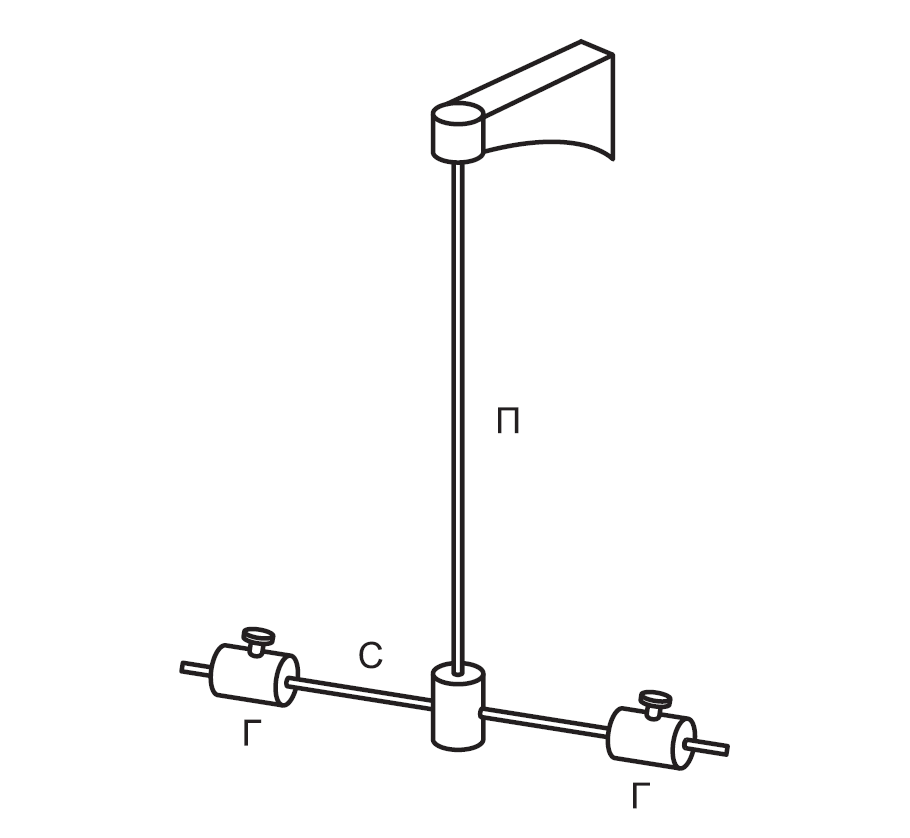
\includegraphics[scale=0.3]{ust2.png}
        \begin{center}
        \caption{Схема установки}
        \end{center}
        \label{graphic1b}
    \end{center}
\end{figure}

\begin{center}
    \subsection*{Ход работы}
\end{center}

\begin{table}[h!]
    \begin{center}
        \begin{tabular}{|c|c|}
        \hline
        Масса груза 1, гр     & 378,0 $\pm$ 0,1 \\ \hline
        Масса груза 2, гр     & 373,0 $\pm$ 0,1 \\ \hline
        Диаметр проволоки, мм & 1,39 $\pm$ 0,01 \\ \hline
        Длина проволоки, мм   & 1730 $\pm$ 2    \\ \hline
        Длина цилиндра, мм    & 48 $\pm$ 0,1    \\ \hline
        \end{tabular}
        \caption{Размеры установки}
    \end{center}
\end{table}

\begin{table}[h!]
    \begin{center}
        \begin{tabular}{|c|c|c|c|}
        \hline \hline
        $l$, см & $n$ & $t$, c & $T, $ c  \\ \hline \hline
        12,35 & 10 & 36,59 & 3,659 \\ \hline
        11,38 & 10 & 33,95 & 3,395 \\ \hline
        10,34 & 10 & 31,26 & 3,126 \\ \hline
        9,34  & 10 & 28,73 & 2,873 \\ \hline
        8,35  & 10 & 26,23 & 2,623 \\ \hline
        7,33  & 10 & 23,70 & 2,370 \\ \hline
        6,32  & 10 & 21,40 & 2,140 \\ \hline
        5,30  & 10 & 19,09 & 1,909 \\ \hline
        4,50  & 10 & 17,49 & 1,749 \\ \hline \hline
        \end{tabular}
        \caption{Экспериментальные данные}
    \end{center}
\end{table}

\begin{figure}[H]
    \centering
    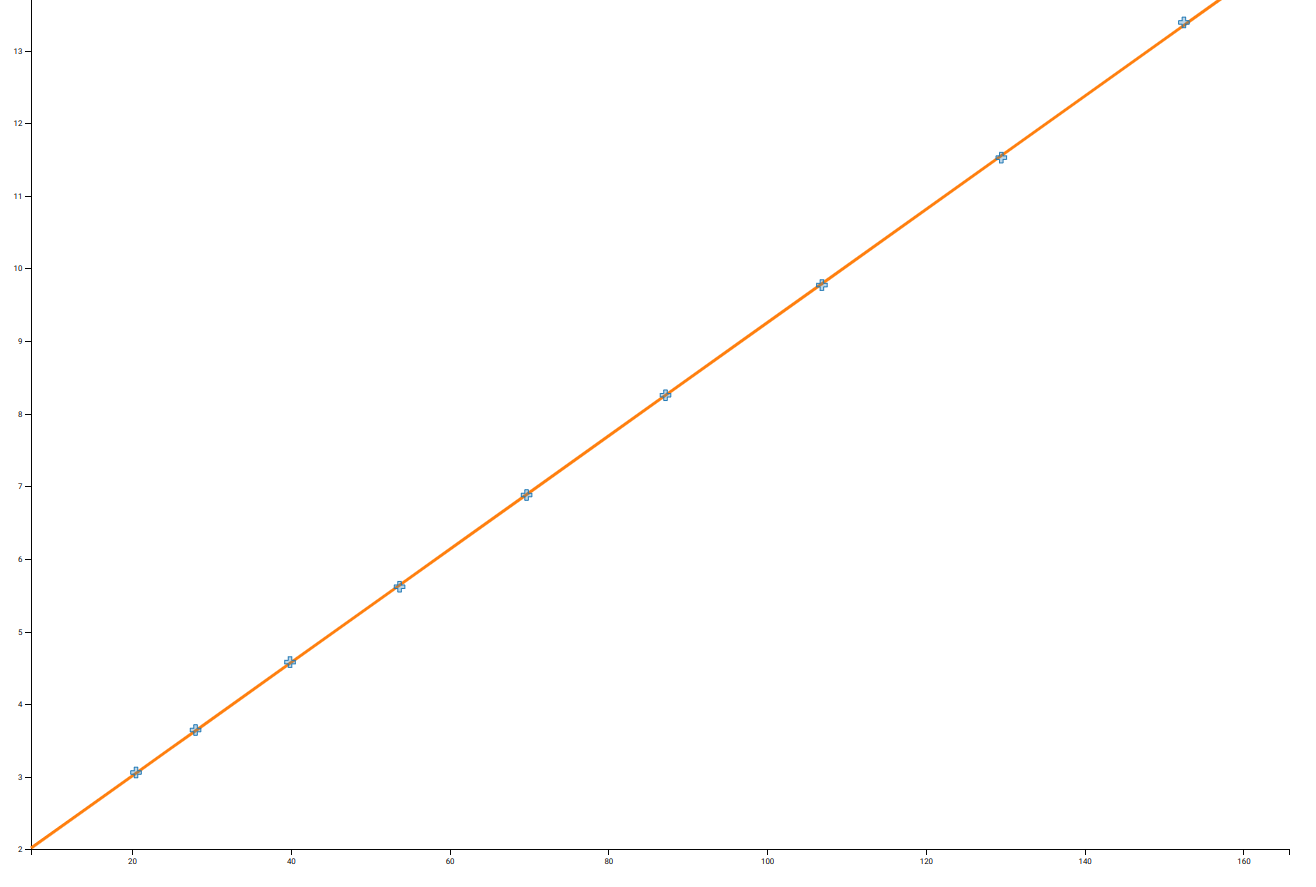
\includegraphics[scale=0.4, angle=90]{graph2.png}
    \caption{Зависимость $T^2 = kl^2 + b$}
\end{figure}

\begin{center}
    Уравнение графика: $y=0.078x+1.449$

    \bigskip

Тогда $k = (0,078 \pm  0,00089), \; \varepsilon_{k} \approx 1,34\%$ $\frac{c^2}{\text{см}^2}$

\begin{equation}    
    f = (2\pi)^2\frac{(m_{1}+m_{2})}{k}
\end{equation}

\newpage

Погрешность:
\[
    \varepsilon_{f} = \sqrt{(\varepsilon_{m_{1}})^2 + (\varepsilon_{m_{2}})^2 + (\varepsilon_{k})^2} 
\]
Получаем $\varepsilon_{f} = 1,35\%$ и $f = 0,0380$ Н $\cdot$ м.\\
\[
    G=\frac{2l}{\pi R^{4}}f
\]
Погрешность:
\[
    \varepsilon_{G} = \sqrt{(\varepsilon_{f})^2 + (\varepsilon_{l})^2 + (4\varepsilon_{R})^2} 
\]
Итого: \underline{$\varepsilon_{G} = 3,16\%$, $G = 17,9 \cdot 10^{10} \frac{\text{Н}}{\text{м}^2}$} 

\end{center}

\begin{center}
    \section*{Вывод}
    Были вычислены модули кручения двумя разными способами и на их основе определены модули сдвига материала.
\end{center}
    
\end{document}
  